\documentclass[a4paper]{article}
\usepackage[14pt]{extsizes} 
\usepackage[T2A]{fontenc}
\usepackage[utf8]{inputenc}
\usepackage{natbib}
\usepackage{graphicx}
\usepackage{amsmath}
\usepackage[english, russian]{babel}
\usepackage{fontspec}
\usepackage{amsmath,amsfonts,amssymb,amsthm,mathtools,mathrsfs}
\usepackage{icomma}
\usepackage{fullpage}
\usepackage{ulem}
\usepackage{eufrak}
\usepackage{setspace}
\usepackage{listings}
\usepackage{indentfirst}
\usepackage[left=2cm,right=1.5cm,top=2cm,bottom=2cm]{geometry}
\usepackage{xcolor}
\usepackage{float}
\usepackage{csquotes}

\setmainfont[Ligatures={TeX,Historic}]{Times New Roman}
\setlength{\parindent}{5ex}
\setlength{\parskip}{1em}
\renewcommand{\baselinestretch}{1}

\graphicspath{{images/}}

\definecolor{buzzlightyear}{HTML}{8757A5}
\definecolor{grass}{HTML}{738D06}
\definecolor{literal}{HTML}{F18A2B}
\definecolor{commentcolor}{HTML}{8E908B}

\lstdefinestyle{habrstyle}{
    backgroundcolor=\color{white},   
    commentstyle=\color{commentcolor},
    keywordstyle=\bfseries\color{buzzlightyear},
    numberstyle=\tiny\color{commentcolor},
    stringstyle=\color{grass},
    basicstyle=\ttfamily\footnotesize,
    breakatwhitespace=false,         
    breaklines=true,                 
    captionpos=b,                    
    keepspaces=true,                 
    numbers=left,                    
    numbersep=5pt,                  
    showspaces=false,                
    showstringspaces=false,
    showtabs=false,                  
    tabsize=4
}

\lstset{style=habrstyle}

\begin{document}
    % НАЧАЛО ТИТУЛЬНОГО ЛИСТА
    \begin{center}
        \begin{center}
        \hfill \break
        \normalsize{Санкт-Петербургский государственный политехнический}\\
        \normalsize{университет Петра Великого}\\
        \hfill \break
        \normalsize{\textbf{Высшая школа интеллектуальных систем и}}\\ 
        \normalsize{\textbf{суперкомпьютерных технологий}}\\ 
        \hfill \break
        \hfill \break
        \hfill \break
        \normalsize{Лабораторная работа}\\
        \hfill \break
        \hfill \break
        \normalsize{\LARGE Автокорреляция}\\
        \end{center}
        \hfill \break
        \hfill \break
        \hfill \break
        \hfill \break
        \hfill \break
        \hfill \break
        \hfill \break
        \hfill \break
        \hfill \break
        \hfill \break
        \begin{flushright}
            \normalsize{Работу выполнил студент}\\
            \normalsize{3-го курса, группа 3530901/80201}\\
            \normalsize{Солянкин Илья Андреевич}\\
            \hfill \break
            \normalsize{Преподаватель:}\\
            \normalsize{Богач Наталья Владимировна}\\
        \end{flushright}
        \hfill \break
        \hfill \break
        \hfill \break
        \hfill \break
        \begin{center} Санкт-Петербург 2021 \end{center}
        \thispagestyle{empty}
    \end{center}
    % КОНЕЦ ТИТУЛЬНОГО ЛИСТА
    
    % ОГЛАВЛЕНИЕ
    \newpage
        \tableofcontents
    
    % СПИСОК ИЛЛЮСТРАЦИЙ
    \newpage
         \listoffigures
    
    % СПИСОК ЛИСТИНГОВ     
    \newpage
         \lstlistoflistings   
     
    \newpage
        \section{Часть №1: Оценка высоты тона вокального чирпа}
            В первом пункте пятой лабораторной работы нам необходимо вычислить автокорреляцию для различных \texttt{Lag} и оценить высоты тона вокального чирпа.
            
            Начнем с написания функции \texttt{serial-corr} и \texttt{autocorr}:
            
\begin{lstlisting}[language=Python, caption= Функция \texttt{serial-corr}]
    def serial_corr(wave, lag=1):
        N = len(wave)
        y1 = wave.ys[lag:]
        y2 = wave.ys[:N-lag]
        corr = np.corrcoef(y1, y2)[0, 1]
        return corr
\end{lstlisting}      

\begin{lstlisting}[language=Python, caption= Функция \texttt{autocorr}]
    def autocorr(wave):
        lags = np.arange(len(wave.ys)//2)
        corrs = [serial_corr(wave, lag) for lag in lags]
        return lags, corrs
\end{lstlisting} 
           
           После этого прочитам чирп с записью голоса и для проверки выведем его:
           
            \begin{figure}[H]
                \centering
                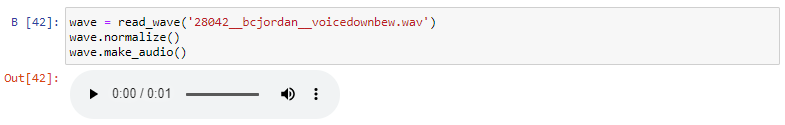
\includegraphics[width=\textwidth]{ex_1_audio.png}
                \caption{Получение чирпа}
                \label{fig:ex_1_audio}
            \end{figure}
           
           После этого построим график автокорреляции:
           
\begin{lstlisting}[language=Python, caption= Построение графика автокорреляции]
    segment = wave.segment(0, 0.01)
    lags, corrs = autocorr(segment)
    lagx = np.array(corrs[90:110]).argmax() + 90
    thinkplot.plot(lags, corrs, color = 'blue')
    thinkplot.config(xlabel='Lag', ylabel='Correlation')
\end{lstlisting}               
            
            \begin{figure}[H]
                \centering
                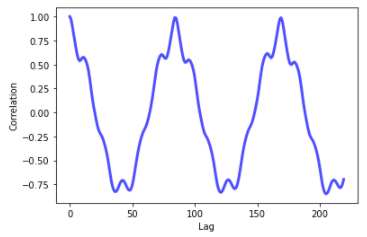
\includegraphics{ex_1_segment.png}
                \caption{Полученный график автокорреляции}
                \label{fig:ex_1_segment}
            \end{figure}
            
            По графику видко, что он периодиечкий, период равен 90 \texttt{Lag}
           
    
    \newpage
        \section{Часть №2: Функция \texttt{estimate-fundamental}}
            Во втором пункте пятой лабораторной рабооты нам необходимо написать функцию \texttt{estimate-fundamental}, отслеживающую высоту тона записанного звука. Также необходимо проверить ее работоспособность.
            
            Для начала напишем функцию \texttt{estimate-fundamental}. которая с помощью функции автокорреляции может помочь в отслеживании высоты тона:
            
\begin{lstlisting}[language=Python, caption= Функция \texttt{estimate-fundamental}]
    def estimate_fundamental(segment, low=70, high=150):
        lags, corrs = autocorr(segment)
        lag = np.array(corrs[low:high]).argmax() + low
        period = lag / segment.framerate
        frequency = 1 / period
        return frequency
\end{lstlisting}
            
            После этого возмем запись чирпа:
            
            \begin{figure}[H]
                \centering
                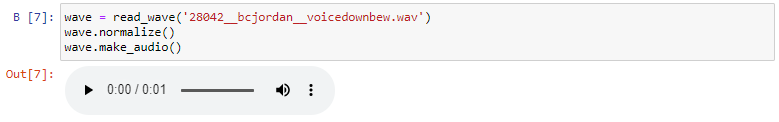
\includegraphics[width=\textwidth]{ex_2_audio.png}
                \caption{Получение чирпа}
                \label{fig:ex_2_audio}
            \end{figure}
            
            Теперь построим спектограмму полученной записи:
            
\begin{lstlisting}[language=Python, caption= Построение спектограммы]
    wave.make_spectrogram(2048).plot(high=4200)
    decorate(xlabel='Time (s)', ylabel='Frequency (Hz)')
\end{lstlisting}               
            
            \begin{figure}[H]
                \centering
                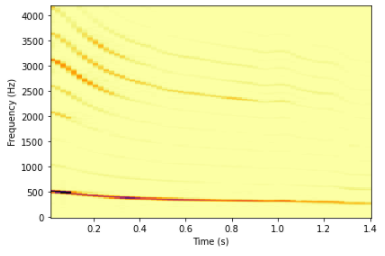
\includegraphics{ex_2_spectogramma.png}
                \caption{Построенная спектограмма}
                \label{fig:ex_2_spectogramma}
            \end{figure}
            
            Затем с помощью написанной ранее функции \texttt{estimate-fundamental} получим частоту минимального сегмента:
            
            \begin{figure}[H]
                \centering
                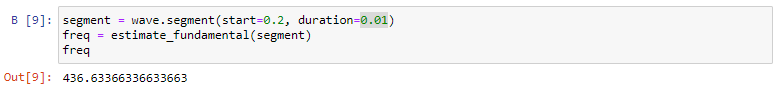
\includegraphics[width=\textwidth]{ex_2_freq.png}
                \caption{Полученная частота минимального сегмента}
                \label{fig:ex_2_audio}
            \end{figure}
            
            ПОсле этого с шагом 0,05 найдем этот сегмент:
            
\begin{lstlisting}[language=Python, caption= Нахождение нужного сегмента]
    starts = np.arange(0.0, 1.4, 0.05)
    ts = []
    freqs = []
    for start in starts:
        ts.append(start + 0.05/2)
        segment = wave.segment(start=start, duration=0.01)
        freq = estimate_fundamental(segment)
        freqs.append(freq)
\end{lstlisting} 
            
            И, наконец, выведем его спектограмму на экран:
            
\begin{lstlisting}[language=Python, caption= Вывод спектограммы сегмента]
    wave.make_spectrogram(2048).plot(high=900)
    plt.plot(ts, freqs, color='white')
    decorate(xlabel='Time (s)', ylabel='Frequency (Hz)')
\end{lstlisting}               
            
            \begin{figure}[H]
                \centering
                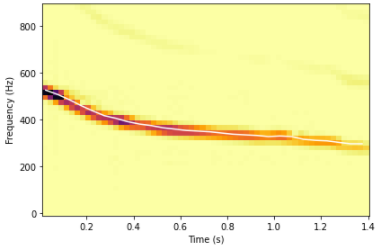
\includegraphics{ex_2_spectogramma_last.png}
                \caption{Построенная спектограмма сегмента}
                \label{fig:ex_2_spectogramma_last}
            \end{figure}
            
            В результате на полученной спектограмме сегмента можно увидеть частоту тона в каждый момент времени

    \newpage
        \section{Часть №3: \texttt{BitCoin}}
            В третьем пункте пятой лабораторной работы нам необходимо использую данные цен \texttt{BitCoin} из прошлой лабораторной работы вычислить автокорреляцию цен на \texttt{BitCoin}.
            
            Возмем тот же файл, что и в прошлой лабораторной работе и так же представим данные из него в виде графика:
            
\begin{lstlisting}[language=Python, caption= Представление данных файла в виде графика]
    df = pd.read_csv('BTC_USD_2013-10-01_2020-03-26-CoinDesk.csv', parse_dates=[0])
    ys = df['Closing Price (USD)']
    ts = df.index
    wave = Wave(ys, ts, framerate=1)
    wave.plot()
    decorate(xlabel='Time (days)', ylabel='Price of BitCoin ($)')
\end{lstlisting}               
            
            \begin{figure}[H]
                \centering
                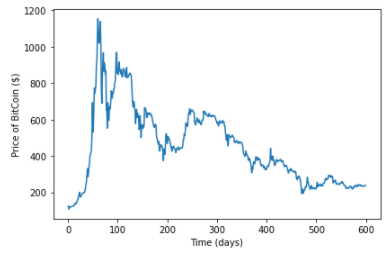
\includegraphics{ex_3_wave_plot.png}
                \caption{Данные из файла в виде графика}
                \label{fig:ex_3_wave_plot}
            \end{figure}
            
            После этого с помощью функции автокорреляции получим еще один график:
            
\begin{lstlisting}[language=Python, caption= Получение нового графика после автокорреляции]
    lags, corrs = autocorr(wave)
    thinkplot.plot(lags, corrs)
    decorate(xlabel='Lag', ylabel='Correlation')
\end{lstlisting}               
            
            \begin{figure}[H]
                \centering
                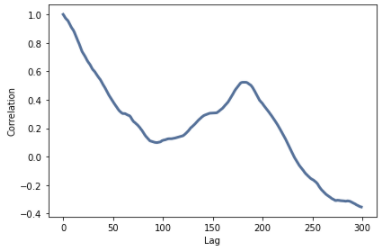
\includegraphics{ex_3_autocorr.png}
                \caption{Полученный график после автокорреляции}
                \label{fig:ex_3_autocorr}
            \end{figure}
            
            В результате можн осказать о том, что полученный график повторяет график цены \texttt{BitCoin}. Периодичность в графике не наблюдается.
            
    \newpage
        \section{Часть №4: \texttt{saxophone.ipynb}}
            В чертвертом пункте пятой лабораторной работы нам необходимо прочитать блокнот \texttt{saxophpne.ipynb}, пройтись по всем примерам, затем выбрать другой сегмент записи и поработать с ним.
            
            Будем использовать звук саксофона, который уже был использован:
            
            \begin{figure}[H]
                \centering
                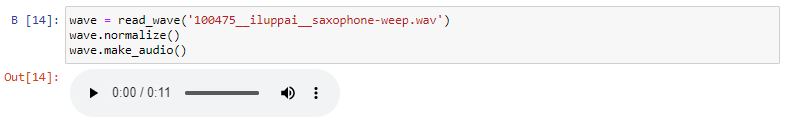
\includegraphics[width=\textwidth]{ex_4_wave_audio.png}
                \caption{Получение звука саксофона}
                \label{fig:ex_4_wave_audio}
            \end{figure}
            
            После этого построим спектограмму данного звука:
            
\begin{lstlisting}[language=Python, caption= Построение спектограммы]
    gram = wave.make_spectrogram(seg_length=1024)
    gram.plot(high=3000)
    decorate(xlabel='Time (s)', ylabel='Frequency (Hz)')
\end{lstlisting}               
            
            \begin{figure}[H]
                \centering
                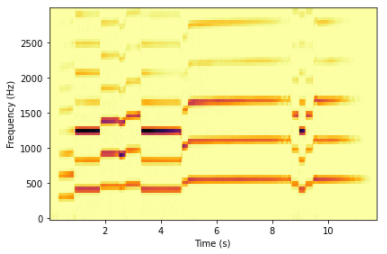
\includegraphics{ex_4_spectogramma.png}
                \caption{Полученная спектограмма}
                \label{fig:ex_4_spectogramma}
            \end{figure}
            
            После этоо выделим сегмент из исходной записи с 6 секунды длительностью 0,5 секунды:
            
            \begin{figure}[H]
                \centering
                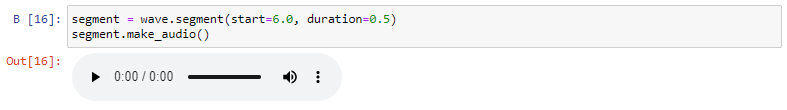
\includegraphics[width=\textwidth]{ex_4_segment_audio.png}
                \caption{Получение сегмента из записи}
                \label{fig:ex_4_segment_audio}
            \end{figure}
            
            Далее получим спектр из данного сегмента:
            
\begin{lstlisting}[language=Python, caption= Получение спектра сегмента]
    spectrum = segment.make_spectrum()
    spectrum.plot(high=3000)
    decorate(xlabel='Frequency (Hz)', ylabel='Amplitude')
\end{lstlisting}               
            
            \begin{figure}[H]
                \centering
                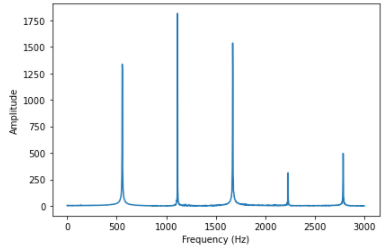
\includegraphics{ex_4_spectr.png}
                \caption{Полученный спектр сегмента}
                \label{fig:ex_4_spectr}
            \end{figure}
            
            Сразу же получим все пики полученного спектра:
            
            \begin{figure}[H]
                \centering
                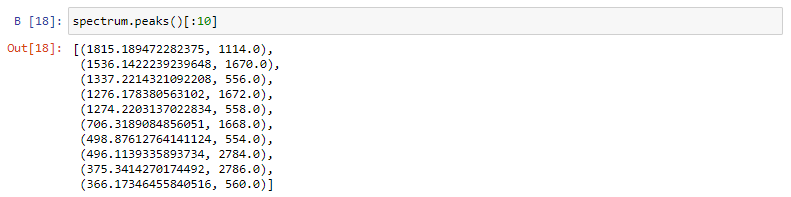
\includegraphics[width=\textwidth]{ex_4_spectr_peaks.png}
                \caption{Пики полученного спектра}
                \label{fig:ex_4_spectr_peaks}
            \end{figure}
            
            Для сравнения получим треугольный сигнал той же частоты:
            
            \begin{figure}[H]
                \centering
                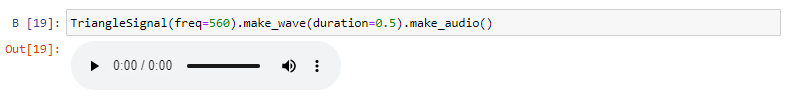
\includegraphics[width=\textwidth]{ex_4_triangle_audio.png}
                \caption{Треугольный сигнал}
                \label{fig:ex_4_triangle_audio}
            \end{figure}
            
            Теперь воспользуемся автокорреляцией для нашего сегмента. Для этого сначала напишем функцию:
            
\begin{lstlisting}[language=Python, caption= Функция для автокорреляции]
    def autocorr(segment):
        corrs = np.correlate(segment.ys, segment.ys, mode='same')
        N = len(corrs)
        lengths = range(N, N//2, -1)
    
        half = corrs[N//2:].copy()
        half /= lengths
        half /= half[0]
        return half
\end{lstlisting}
            
            Теперь обратимся к этой функции и выведем на экран полученный график:
            
\begin{lstlisting}[language=Python, caption= Получение графика автокорреляции]
    corrs = autocorr(segment)
    plt.plot(corrs[:200])
    decorate(xlabel='Lag', ylabel='Correlation', ylim=[-1.05, 1.05])
\end{lstlisting}               
            
            \begin{figure}[H]
                \centering
                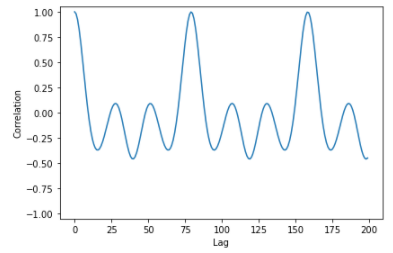
\includegraphics{ex_4_spectr_autocorr.png}
                \caption{Полученный график автокорреляции}
                \label{fig:ex_4_spectr_autocorr}
            \end{figure}
            
            По графику видно, что первый наибольший пик начинается приверно около \texttt{lag} = 65. Для нахождения частоты в данном \texttt{lag} напишем функцию:
            
\begin{lstlisting}[language=Python, caption= Функция для нахождения частоты]
    def find_frequency(corrs, low, high):
        lag = np.array(corrs[low:high]).argmax() + low
        print(lag)
        period = lag / segment.framerate
        frequency = 1 / period
        return frequency
\end{lstlisting}   
            
            После этого вызовем ее, передав на вход примерные значения начала и конца \texttt{lag}:
            
            \begin{figure}[H]
                \centering
                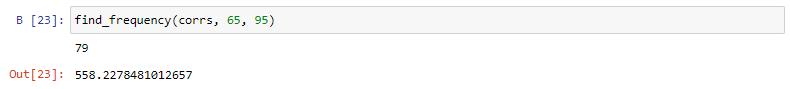
\includegraphics[width=\textwidth]{ex_4_freq.png}
                \caption{Использование написанной функции}
                \label{fig:ex_4_freq}
            \end{figure}
            
            Как можн оувидеть, пик находится на \texttt{lag} = 79
            
            Теперь нам необходимо отфильтровать наш сегмент через фильтр низких частот:
            
\begin{lstlisting}[language=Python, caption= Фильтрация сегмента]
    spectrum2 = segment.make_spectrum()
    spectrum2.high_pass(600)
    spectrum2.plot(high=3000)
    decorate(xlabel='Frequency (Hz)', ylabel='Amplitude')
\end{lstlisting}               
            
            \begin{figure}[H]
                \centering
                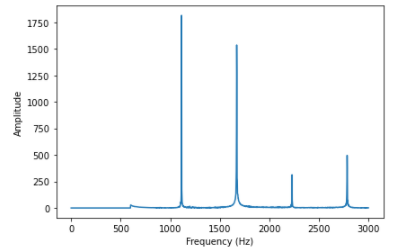
\includegraphics{ex_4_filter_spectr.png}
                \caption{Полученный график после фильтрации}
                \label{fig:ex_4_filter_spectr}
            \end{figure}
            
            Как можн оувидеть по графику, главная частота была убрана.
            
            Теперь нам осталось преобразовать сегмент в аудио для сравнения с исходным сегментом:
            
            \begin{figure}[H]
                \centering
                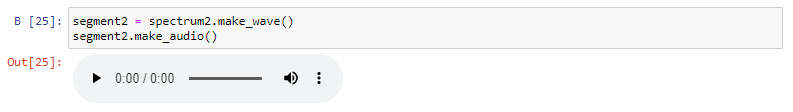
\includegraphics[width=\textwidth]{ex_4_spectr_2_audio.png}
                \caption{Получение аудио из отфильтрованного сегмента}
                \label{fig:ex_4_spectr_2_audio}
            \end{figure}
            
            Наконец, прослушав исходный сегмент и отфильтрованный можно сказать, что эти сигналы очень похожи, но отфильтрованный звучит приглушеннее.
            
    \newpage
        \section{Выводы}
            В результате выполнения данной лабораторной работы мы изучили, что такое автокорреляция. Научились вычислять ее для различных\texttt{lag}. Была создана функция \texttt{estimate-fundamental} для отслеживания вытсоты тона звука. Также вычислили автокорреляцию цен за \texttt{BitCoin} из прошлой лабораторной работы. Наконец, мы поработали с сегментами записи звуков саксофона и вычислили для них автокорреляцию.
           
           
            
\end{document}
